\documentclass{article}
\usepackage[utf8]{inputenc}
\usepackage{graphicx}
\usepackage{hyperref}
\usepackage{xcolor}
\usepackage{fancyvrb}
\usepackage{multicol}
\hypersetup{
    colorlinks,
    linkcolor={red!50!black},
    citecolor={blue!50!black},
    urlcolor={blue!80!black}
}
\usepackage[
backend=biber,
style=alphabetic,
citestyle=authoryear
]{biblatex}
\usepackage{amsmath}
\usepackage{geometry}
 \geometry{
 a4paper,
 total={170mm,257mm},
 left=20mm,
 top=20mm,
 }
% \addbibresource{name.bib} %Imports bibliography file
\setlength\parindent{0pt}

\title{COMP 762 Project Proposal: TraceJump}
\author{David Venuto, Breandan Considine, Pierre Orhan}
\date{October 2019}

\begin{document}

\maketitle
\begin{multicols}{2}
[
\section{Introduction}
]
When operating a computer, it is frequently necessary to copy and paste or manually transcribe text into a search engine. In software development, this activity is especially common. For example, when using an unfamiliar API or programming language, a software developer is likely to seek information such as documentation, code samples, stack traces and bug reports on their favorite search engine. This requires frequently switching contexts between the programming environment and web browser. We consider an information retrieval tool which aides in the navigation and discovery of relevant pages. Consider the following scenario, illustrated in figure:

\begin{enumerate}
    \item User activates the tool.
    \item Screen is annotated with trace links.
    \item User selects a link, which returns a preview of K most relevant documents.
    \item User selects a relevant entry from menu.
    \item URL is opened in the browser.
\end{enumerate}

Our proposed contribution is threefold:

\begin{enumerate}
\item A tool which is capable of annotating text in arbitrary screenshots.
\item Which can suggest relevant developer documents from a corpus.
\item Whose suggestions are adapted to the user's navigation history.
\end{enumerate}

% https://docs.google.com/document/d/1JcgSad7TScVa6Sw6_tpR7UEiSUgMSJECU8kZdeAB0rs/edit?usp=sharing


\section{Scope and research questions}

To narrow down the scope of the project, we impose the following restrictions:

\begin{enumerate}
    \item Start with project one programming language (Java)
    \item Consider source code and natural language web document.
    \item Restrict the evaluation to the code within IDE.
    \item Restrict dataset of source code to source code of API.
    \item Consider only query against:
    \{class, modules, functions, class parameters, global variable \}
\end{enumerate}
Our key idea is to see if a simple framework based on known architecture and trained model of neural network might produce semantically relevant results. We will explore two directions. 

\begin{itemize}
    \item One is to see if we can improve or modify the architecture, for example by proposing a shared latent space as a graph, where each node represents a specific possible output.
    \item The second is to develop a reinforcement learning framework, which leverages the user history to suggest more specific recommendations based on prior user queries.
\end{itemize}.

\subsection{Supervisied learning RQs}

Most of the models we will use are based on the auto-encoder. These models should learn a latent space that encodes their input. Yet, for this to work a few considerations should be highlighted. First we need to restrict the context window these model will use. Similarly, the query context should come from a similar distribution as the training samples from the source code of the API. Next, we need to find a common latent space to represent various kind of programming related content. For this, multiple strategies are possible. One is presented in figure \ref{fig:Orga2}, but we will probably explore others.
The key question for the encoding are thus:
\begin{itemize}
    \item Which fragmentation of the code should we use?
    \item Which latent space should we use to compare queries?
    \item Is it interesting to merge all possible encoding model: code$\xrightarrow{}$latent, NL $\xrightarrow{}$ latent, image$\xrightarrow{}$latent, and then make a nearest neighbor search in this latent space?
    \item Is it interesting to use intermediate representation as suggested in figure \ref{fig:Orga2}: code$\xrightarrow{}$NL$\xrightarrow{}$latent, thus making sure the latent space is the output of a single model (the NL$\xrightarrow{}$latent one)?
\end{itemize}

\subsection{User interaction RQs}

Our reinforcement learning system will be responsible for ranking the results according to a relevancy score. This will depend on a  neural network encoding: \{various database, index: latent space$\xrightarrow{}$Database, queries.
We suggest a first approach in figure \ref{fig:Orga2}: we could first combine a weight for each indexed element to the distance to provide a rank. On such linear approach, different heuristics can be used. Should we only reinforce the weight someone has visited? Should we reinforce all weights coming from the same category? These are some of the questions we hope to answer.
There is no clear answer here, and we need to understand what will be the best for the user.

\end{multicols}
\section{Data preparation}
For our initial dataset, we use the \href{https://zealusercontributions.now.sh/}{Zeal User Contributed docsets}, a collection of documentation for libraries in various programming languages. This dataset contains many links in the following form:

\begin{verbatim}[fontsize=\small]
> grep -oEr "href=\".*?[A-Za-z._-]*\.html\">.*?</a>" . | grep -v ".*http.*"
...
./type_info.html:href="torch.html">torch</a>
./type_info.html:href="tensors.html">torch.Tensor</a>
./type_info.html:href="tensor_attributes.html">Tensor Attributes</a>
./type_info.html:href="sparse.html">torch.sparse</a>
...
\end{verbatim}

The same result, in a more legible format (\texttt{SOURCE\_FILE, LINK\_TARGET, TEXT}):

\begin{verbatim}[fontsize=\small]
> ... sed 's/:/, /g; s/href="//; s/">/, /; s/<\/a>//'
...
./type_info.html, torch.html, torch
./type_info.html, tensors.html, torch.Tensor
./type_info.html, tensor_attributes.html, Tensor Attributes
./type_info.html, sparse.html, torch.sparse
...
\end{verbatim}

We can then compute some statistics for each project:

\begin{verbatim}[fontsize=\small]
> q -Hd , "SELECT text, link_target, COUNT(*) FROM ./data.csv 
  GROUP BY text, link_target ORDER BY COUNT(*) DESC"
Docs,index.html,495
torch,torch.html,280
torch.autograd,autograd.html,171
torch.cuda,cuda.html,170
torch.multiprocessing,multiprocessing.html,167
torch.onnx,onnx.html,167
...
\end{verbatim}

In addition, we include surrounding context in the source and target, document as well as more granular link types extracted from \href{https://en.wikipedia.org/wiki/Fragment_identifier}{fragment identifiers}.

We propose the following preprocessing pipeline:

\begin{enumerate}
    \item Extract links, surrounding context and source document location.
    \item Remove hyperlinks pointing to external URLs.
    \item Resolve fully qualified target document path.
    \item Extract context (e.g. keywords) from target document.
\end{enumerate}

The following schema is proposed: \texttt{SOURCE\_FILE}, \texttt{TARGET\_URL}, \texttt{SOURCE\_TEXT}, \texttt{SOURCE\_TEXT\_PREVIOUS\_N}, \texttt{SOURCE\_TEXT\_NEXT\_N}, \texttt{TOP\_TFIDF\_TARGET\_KEYWORDS}. We note the bipartite structure of the source and target graph -- as the source text is often a single identifier, and the target is often a large document, some feature engineering is necessary to infer links from the source text alone. For simplicity, we use textual adjacency in the source document, and bag-of-words in the target document to provide surrounding context.

We can represent hyperlinks in programming documentation as a directed graph \textit{within} documentation, however our application is primarily intended for predicting links \textit{from} source code \textit{to} documentation. One question we hope to answer is whether links from documentation alone are sufficient to predict relevant trace links in other content types, or whether additional information is required to predict contextually relevant queries.

\begin{multicols}{2}
\subsection{Software architecture}

The proposed workflow requires processing and indexing documents by their constituent keywords. When a query is performed, our goal is to return both documents which contain specific keyword matches, as well as those which contain semantically related text. We believe it will be advantageous to incorporate both classical information retrieval tools, as well as embedding-based semantic search. Two candidates are evaluated for performing keyword search and semantic search, respectively: \href{https://lucene.apache.org/core/}{Apache Lucene} and \href{https://gnes.ai/}{GNES} (Generic Neural Elastic Search). In the information retrieval literature, Lucene is a widely used tool for text indexing. GNES is a relatively modern tool based on the BERT language model. We hope to evaluate the latency and accuracy of these two tools as a baseline, alongside our models.

\section{Model architecture}

Our classification model will rely on two steps.

\begin{enumerate}
    \item  The first step is an unsupervised method to select a short candidate list of links for display to the user.  This method relies on learning a latent space of all the features extracted from documentation and user code (IDE interactions).  The latent space will be learned through an auto-encoder framework.  We will then perform a $k$-nearest neighbour selection  to determine the top $k$ candidate documents to recommend.

\item The second part of the model will consist of a supervised learning framework that is used to predict which link the user is most likely to use given from the short candidate list. We plan to consider a large feature set of user interaction attributes including the query text, the code surrounding the query text and the actions that the user recently performed in the IDE.  

\end{enumerate}

The unsupervised learning framework will likely be a VAE (latent variables are extracted) as a form of dimensionality reduction.  We will use a simple feature space than in (2), likely only query and code-text features. % PROBLEM HERE??

The supervised learning framework (2) will consist of a word embedding input.  We will further extract features with a CNN layer and the feed this as input to a bidirectional LSTM. The output will be concatenated with any other features, producing a softmax over all candidate targets.

\section{Prior work}

We provide here an extensive link of paper we have drawn inspiration form. A more structured background summary will be provided in the final paper.
We used a 
\href{https://ml4code.github.io/}{repository of paper on ML and NLP} to guide our background review.
\begin{enumerate}
    \item \href{https://ml4code.github.io/publications/chen2019literature/}{A review on embedding on source code lead us to the following.} :
        \begin{enumerate}
            \item \href{https://ieeexplore-ieee-org.proxy3.library.mcgill.ca/document/7985683}{Exploring API Embedding for API Usages and Applications}: This work uses Word2Vec to generate API vector from sequence of API code. Then it uses these vectors to map to  similar API code in another language.
            \item \href{https://arxiv.org/pdf/1605.08535.pdf}{DeepAPI} generate API sequences from a given text by using word embeddings and RNN Encoder-Decoder. We inspired from this work to design our architecture as of figure \ref{fig:Orga2}, but completely reversed their design: we go from API sequences, and more generally source code to a text description. The author provide an interesting way to obtain data pairs (sequence,text) that we might use additionally.
            \item \href{https://www.researchgate.net/publication/296526040_From_Word_Embeddings_To_Document_Similarities_for_Improved_Information_Retrieval_in_Software_Engineering}{Word Embedding to document similarities.} Skip-gram model on API and reference documents and tutorials to create embedding for words and code
elements.
        \end{enumerate}
    \item \href{https://miltos.allamanis.com/publicationfiles/allamanis2018survey/allamanis2018survey.pdf}{Review on ML for big code}, Especially part 5.1 on recommender systems, is of our interest. 
    Simply put: recommender systems focused on code completion or code code reviewer. Some author have tried to provide ranked lists:
        \begin{enumerate}
            \item \href{https://hal.archives-ouvertes.fr/hal-01575348/file/Learning-from-Examples-to-Improve-Code-Completion-Systems.pdf}{Bruch at al} Extracted feature from code context to suggest completions for method invocations and constructors
            \item \href{http://www.st.informatik.tu-darmstadt.de/artifacts/pbn/proksch-2015-Intelligent-Code-Completion-with-Bayesian-Networks.pdf}{Proksch} Code completion with Bayesian graphical models. A bit far from our work...
        \end{enumerate}
    \item \href{https://arxiv.org/pdf/1810.08305.pdf}{Open vocabulary learning on source code with a graph-structured cache} Builds on graph neural network to understand fast-vocabulary changing. We might use some of these strategies in a second round of improvements of our architecture.
    \item \href{http://citeseerx.ist.psu.edu/viewdoc/download?doi=10.1.1.722.150&rep=rep1&type=pdf}{Graph-based statistical language model for Code} Learn from a source code corpus and compute the appearance probabilities of any graphs given observed subgraphs. Model are called "GraLan" and "ASTLan". This work is based on their previous work where they introduced the GROUM model, which suggests a way to design a graph on source code : \href{https://www.researchgate.net/publication/221560251_Graph-based_mining_of_multiple_object_usage_patterns}{Graph based mining of multiple object usage patterns} (2009)
    \item On API mining for recommendations:
        \begin{enumerate}
            \item \href{https://homepages.inf.ed.ac.uk/csutton/publications/fse2016.pdf}{Parameter-free probabilistic API mining across GitHub} Insists on the fact that frequentist approach are not that great. The approach is parameter-free, which is nice. This might give us intuition to build a second more evolved model.
            \item \href{https://www.researchgate.net/publication/221115320_SNIFF_A_Search_Engine_for_Java_Using_Free-Form_Queries}{SNIFF}, finds abstract code examples relevant to a natural language query expressing a desired task. Annotates available source code with API documentation and the annotated code is then indexed for searching. Syntax-aware intersection, clustered and ranked based on frequency occurrences.
            \item \href{http://post.queensu.ca/~zouy/files/icse2014.pdf}{Keivanloo et al.} find abstract code examples by combining textual similarity and clone detection techniques, ranking by \{similarity to query, completeness, popularity of concrete usage patterns\} Yet very focused on finding a "working example"
            \item \href{https://www.cs.ubc.ca/~rtholmes/papers/icse_2005_holmes.pdf}{Strathcona}: code example recommendation. First generates a query given the code context, then use 6 heuristics comparing structural context of the classes and methods with an example repository. Ranking: frequency in final set of examples returned by each heuristics.  Interesting, but very focused on building an example repo, which we considered to all-ready have. Yet very similar in the human interaction ideas.
          \end{enumerate}
    These older works are focused on feature design.
    \item On other API mining:
        \begin{enumerate}
            \item \href{http://web.cs.iastate.edu/~design/papers/ICSE-13/icse13.pdf}{BOA} tool/language for large scale mining of software repository... \item \href{http://design.cs.iastate.edu/papers/ICSE-14/icse14.pdf}{Mining Billions of AST Nodes to Study Actual and Potential Usage of Java Language Features} mine existing code to measure popularity of language constructs and APIs. (used BOA)
        \end{enumerate}
\end{enumerate}

\section{Author contributions} % LET'S KEEP THIS UPDATED

David designed and performed the learning experiments. Breandan collected the dataset and wrote the user interaction tool. Pierre contributed to the architecture and UI design and literature review.

\printbibliography

\end{multicols}

\begin{figure}
    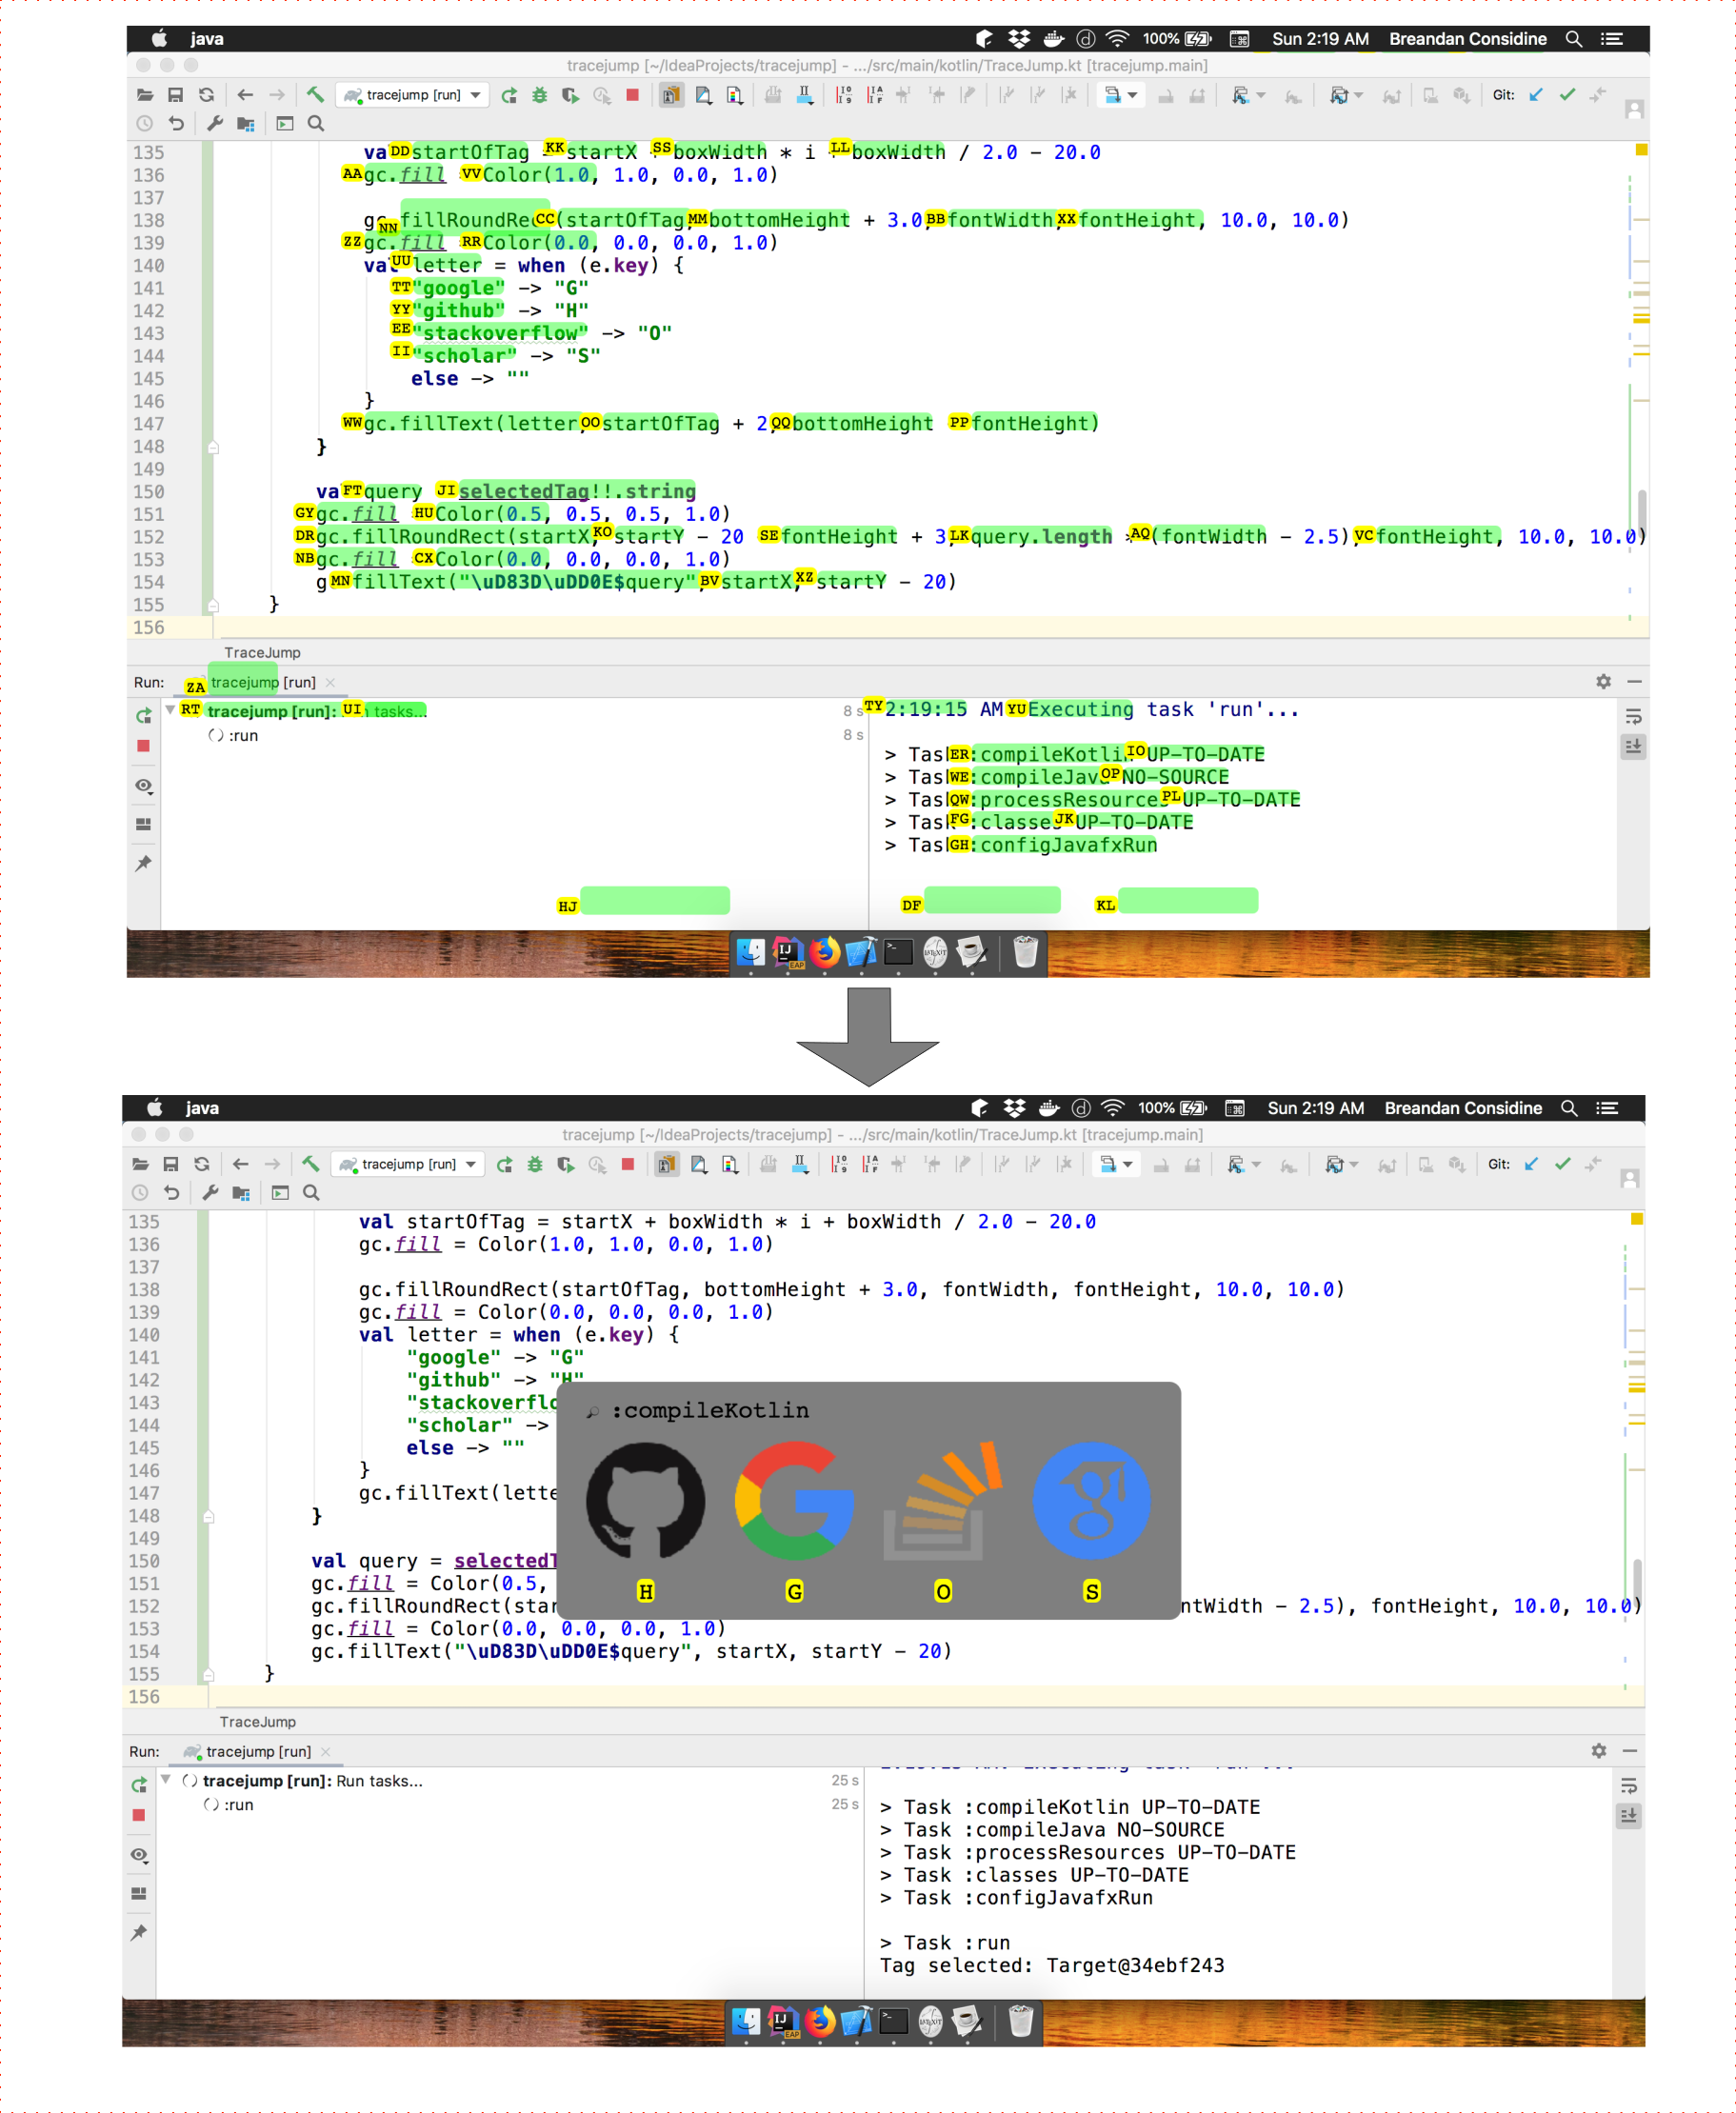
\includegraphics[width=\textwidth]{BreandanTool.png}
    \caption{User interaction with the tool. }
    \label{fig:my_label}
\end{figure}
\begin{figure}
    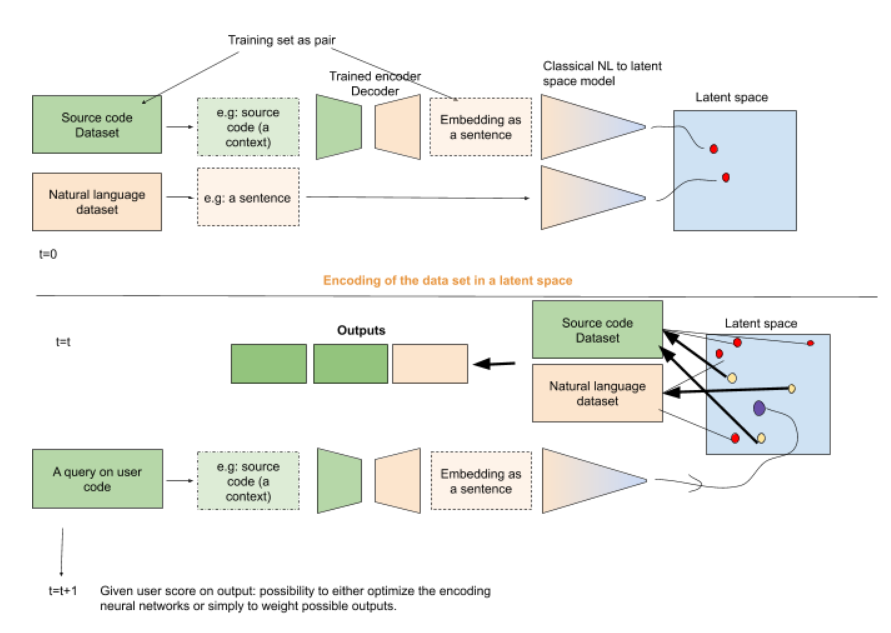
\includegraphics[width=\textwidth]{toolOrga2.PNG}
    \caption{Proposition for the tool structure. There is two model, one that encode source code and decodes it into a sentence embedding. The second is a pre-trained model that corresponds to the embedding from a sentence into a latent space.}
    \label{fig:Orga2}
\end{figure}

\end{document}